%% ============================================================================
%% Frontiers in Digital Health - Manuscript
%% Following format of Ricciardi et al. (2024) Frontiers in Digital Health
%% Title: Machine Learning for Emergency Department Length of Stay, 
%%        Admission, and Hospitalization Prediction Using Triage-Only Data
%% ============================================================================

\documentclass[harvard,article]{frontiersinFPHY_FAMS}

\usepackage{url,lineno,amsmath,amssymb,graphicx}
\usepackage{booktabs,multirow,tabularx,caption,subcaption,float}
\usepackage{array}
\usepackage[colorlinks=true, urlcolor=blue, citecolor=black, linkcolor=black]{hyperref}

\linenumbers
\onecolumn

\def\keyFont{\fontsize{8}{11}{\helveticabold}}
\def\firstAuthorLast{Onwurah {et~al.}}

\title{Machine Learning for Emergency Department Length of Stay, Admission, and Hospitalization Prediction Using Triage-Only Data}

\author{Onyedikachi I. Onwurah$^{1}$, Sol Richardson$^{1}$, Sheng Wu$^{2}$, and  Tong Xia$^{1,*}$ \\
\vspace{0.2cm}
\small{$^{1}$Vanke School of Public Health, Tsinghua University, Beijing, China}\\
\small{$^{2}$Beijing Tsinghua Changgung Hospital, Beijing, China} \\
}
\correspondance{Tong Xia$^{1,*}$: tongxia@tsinghua.edu.cn}

\begin{document}

\maketitle

% ============================================================================
% ABSTRACT
% ============================================================================
\begin{abstract}

\noindent\textbf{Background:} Emergency Department (ED) crowding is a critical public health challenge. Prolonged boarding ($\geq$8 hours) affects over 20\% of visits. Hospital admission and prolonged hospitalization ($>$7 days) consume disproportionate resources. Clinicians currently rely on triage scales like the Emergency Severity Index (ESI), which have limited predictive accuracy. Machine learning (ML) using triage-only data could support these decisions, but evidence on model accuracy remains limited.

\noindent\textbf{Methods:} Using the MC-MED dataset (118,385 adult ED visits), we evaluated four ML models (XGBoost, LightGBM, Random Forest, TabNet) on three binary classification tasks using 29 admission-available variables: (1) predicting prolonged ED length of stay (ED-LOS $\geq$8 hours vs. $<$8 hours), (2) predicting hospital admission (admit vs. discharge), and (3) predicting prolonged hospital length of stay (hospital LOS $>$7 days vs. $\leq$7 days) among admitted patients. All 29 features were available within 90 minutes of arrival. Area under the receiver operating characteristic curve (AUC-ROC) was the primary performance metric. SHAP (SHapley Additive exPlanations) analysis identified the most important features for each prediction task.

\noindent\textbf{Results:} For ED-LOS $\geq$8 hours, XGBoost achieved an AUC-ROC of 0.660 (95\% CI: 0.652-0.668). For hospital admission, XGBoost achieved an AUC-ROC of 0.817 (95\% confidence interval [CI]: 0.810-0.824), an improvement over the ESI baseline of 0.678. For hospital LOS $>$7 days among admitted patients, Random Forest achieved an AUC-ROC of 0.671 (95\% CI: 0.662-0.680). SHAP analysis identified consistent top predictors across tasks: triage acuity, emergency medical services (EMS) arrival, age, disease condition count, and the Charlson Comorbidity Index.

\noindent\textbf{Conclusion:} ML using only triage-available data accurately predicts three critical ED binary treatment outcomes. SHAP analysis provides interpretable feature importance to support clinical decision-making.
\end{abstract}
\noindent\textbf{Keywords:} machine learning, emergency department, hospital admission, length of stay, Shapley Additive Explanations

% ============================================================================
% INTRODUCTION
% ============================================================================
\section{INTRODUCTION}

Emergency departments (EDs) offer a fundamental service, providing emergency treatments 24 hours a day, 365 days a year, therefore representing a critical public health service role \cite{higginson2012, trzeciak2003, ricciardi2024}. Crowding in EDs has been recognised as a critical challenge in hospital administration \cite{asplin2003, rcem2025}. ED crowding has been linked to increased costs, longer waiting times, higher mortality rates, and adverse outcomes for vulnerable populations \cite{sun2013, burke2020, obermeyer2019}.

The length of stay in the ED (ED-LOS) is a significant indicator of ED bottlenecks. ED-LOS is defined as the interval from ED arrival to ED departure \cite{stone2022, ricciardi2024}. A prolonged ED-LOS is a consequence of crowding and has been associated with a 37\% elevated mortality risk among admitted patients \cite{sun2013}. Several studies have defined an extended ED-LOS as more than 3 hours \cite{ricciardi2024}, while others use thresholds of 4 to 12 hours \cite{farimani2024}. Prolonged boarding not only affects patient outcomes but also contributes to ambulance diversion, treatment delays for time-sensitive conditions, and inefficient resource utilization across the hospital system.

Clinicians currently rely on triage scales such as the Emergency Severity Index (ESI) to prioritize patients and predict clinical trajectories. However, the ESI demonstrates limited predictive accuracy for key outcomes such as hospital admission and prolonged length of stay when used in isolation, with AUC-ROC values typically below 0.70 \cite{levin2020}. This limitation creates an opportunity for data-driven approaches that integrate multiple patient characteristics available at triage.

Machine learning (ML) techniques are frequently used in healthcare for diagnosis, forecasting patient outcomes, and resource allocation \cite{kareemi2020, raita2019}. Following this approach, many researchers have examined ways to predict ED-LOS, hospital admission, and hospital LOS using ML strategies \cite{wu2025, fenn2021, lin2024}. Ricciardi et al. \cite{ricciardi2024} achieved 74.8\% accuracy for predicting ED-LOS greater than 3 hours using Random Forest. Wu et al. \cite{wu2025} found that LightGBM outperformed other models for continuous ED-LOS prediction in a Chinese hospital setting.

However, existing models have three critical limitations. First, most studies predict ED-LOS, hospital admission, or hospital LOS in isolation, despite their clinical interdependence in real-world emergency care pathways \cite{stone2022}. Second, many models incorporate laboratory results or specialist consultations that are unavailable at triage, limiting real-time clinical applicability \cite{levin2020}. Third, insufficient interpretability validation beyond single-model SHAP analysis raises concerns about algorithm-specific artifacts versus true clinical signals \cite{slack2022, wang2025}.

Based on these considerations, the aim of this work is to build a predictive model to forecast three binary treatment outcomes using only triage-available variables: (1) prolonged ED-LOS (8 hours or more), (2) hospital admission, and (3) prolonged hospital LOS (more than 7 days) among admitted patients.

Using the MC-MED dataset (118,385 adult ED visits from Stanford Health Care, 2020-2022), we evaluated four ML algorithms (XGBoost, LightGBM, Random Forest, TabNet) on three binary classification tasks using 29 admission-available variables. Our models achieved AUC-ROC values of 0.660 (95\% CI: 0.652-0.668) for ED-LOS $\geq$8 hours, 0.817 (95\% CI: 0.810-0.824) for hospital admission (improving upon the ESI baseline of 0.678), and 0.671 (95\% CI: 0.662-0.680) for hospital LOS $>$7 days among admitted patients. SHAP analysis identified triage acuity, EMS arrival, age, disease condition count, and the Charlson Comorbidity Index as the most important predictors across all tasks. Predicting these outcomes in advance would be beneficial for planning staff allocation and bed management with the goal of reducing ED crowding.

% ============================================================================
% METHODS
% ============================================================================
\section{METHODS}

\subsection{Context and Data Collection}

This study analysed the MC-MED dataset \cite{kansal2025, kansal2025b}, which contains 118,385 adult ED visits from Stanford Health Care between January 2020 and December 2022. The dataset includes demographics, triage vital signs, chief complaints, comorbidity measures, home medications, and visit outcomes \cite{goldberger2000}.

\textbf{Figure 1} shows the data preprocessing pipeline. The pipeline consisted of five stages: (1) raw data loading from the MC-MED dataset (118,385 adult ED visits, 2020-2022), (2) chronological split into training (78\%), validation (11\%), and test (11\%) sets, (3) missing data handling using median, mode, and Multiple Imputation by Chained Equations (MICE), (4) outcome separation where ED-LOS, Hosp-LOS, disposition, and arrival time columns are removed from features before model training to prevent temporal leakage, and (5) binary classification target definition for three tasks: ED-LOS $\geq$8 hours, hospital admission, and Hosp-LOS $>$7 days (among admitted patients only, with filtering of 48,855 discharged patients representing 60.0\% of the training set).

\begin{figure}[H]
\centering
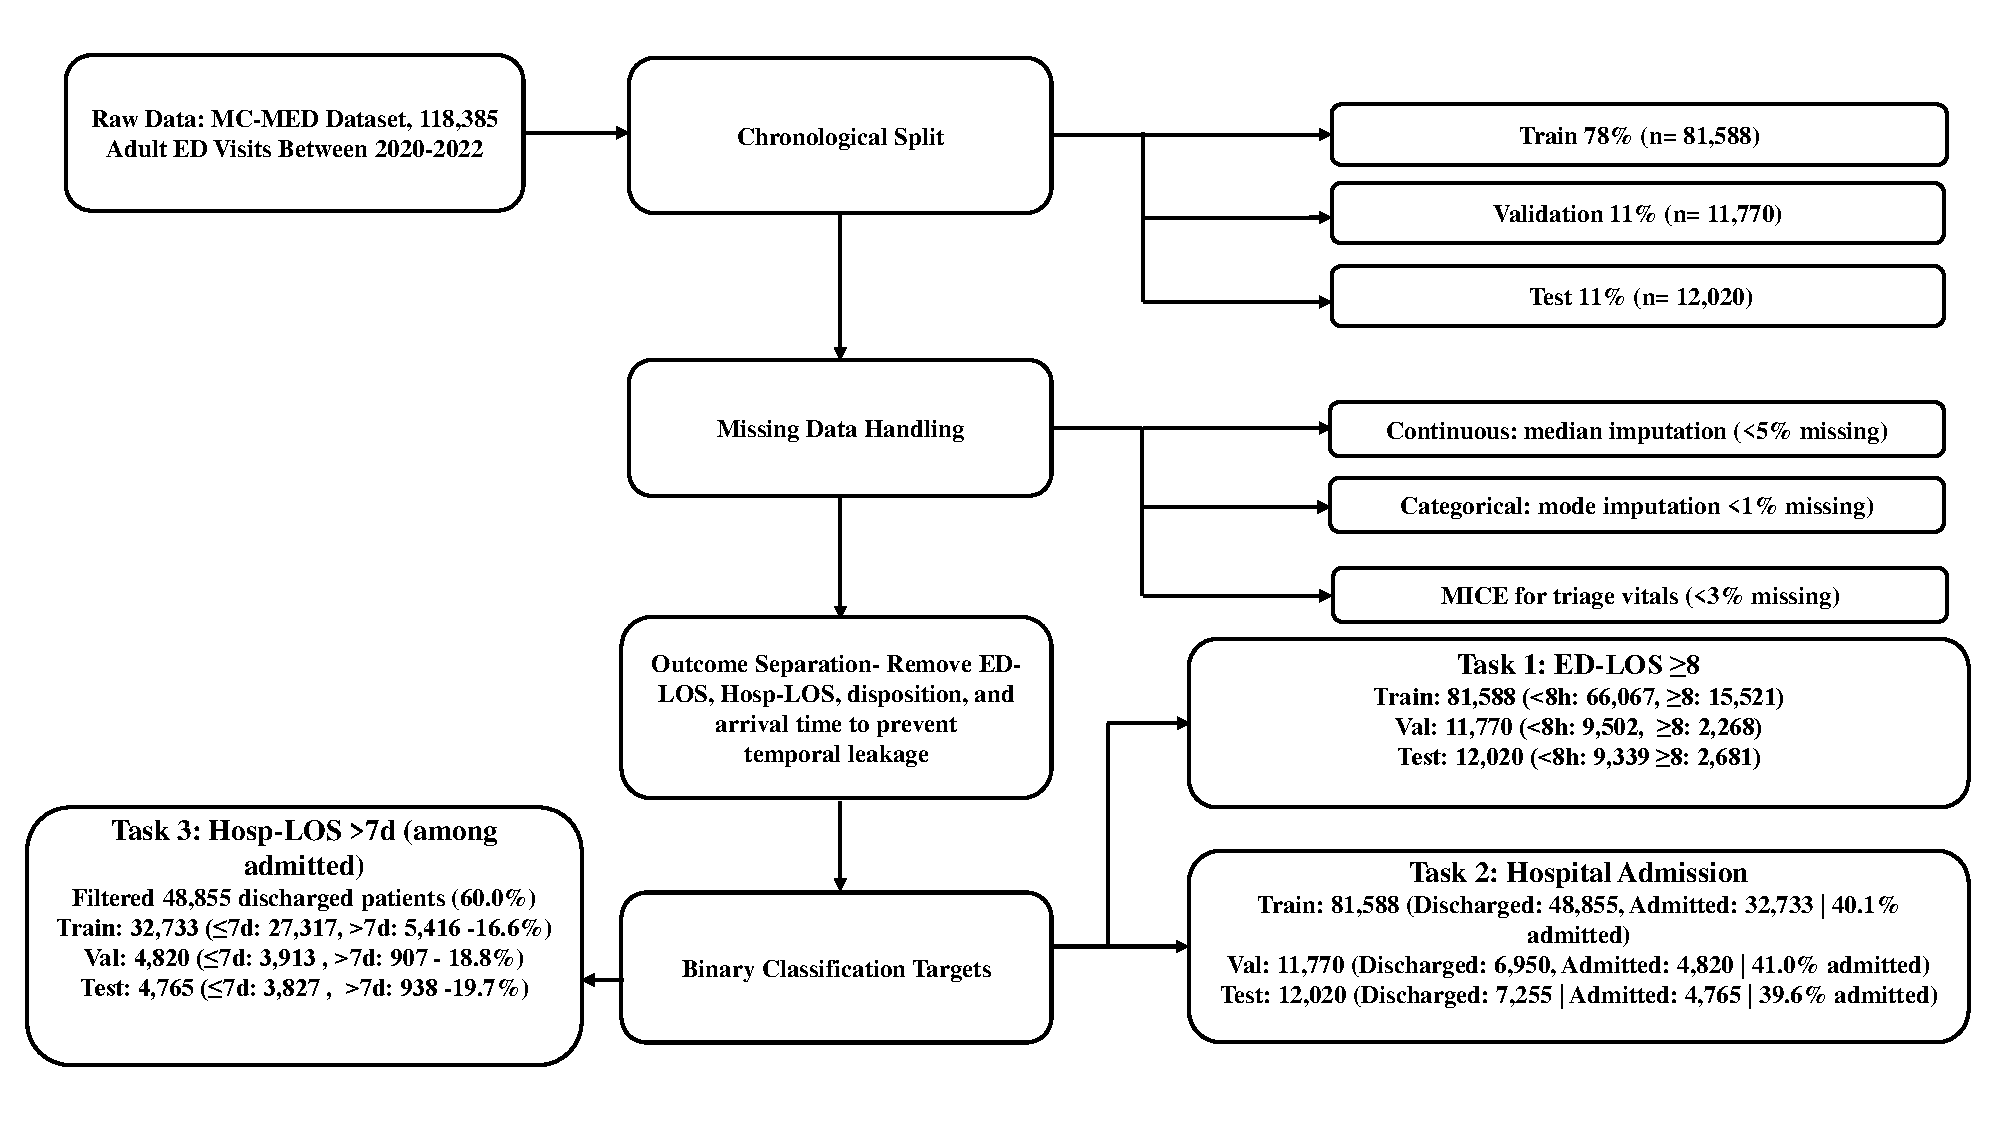
\includegraphics[width=0.95\textwidth]{data preprocessing2.pdf}
\caption{Chronological preprocessing pipeline for the MC-MED dataset showing split proportions, missing data handling methods (median, mode, MICE), outcome separation, and three binary classification targets.}
\label{fig:pipeline}
\end{figure}

Table~\ref{tab:descriptive} presents the demographic and clinical characteristics of the study cohort across the three chronological splits. The mean age was 52.3 years (SD: 19.8), with female patients accounting for 52.1\% of visits. The baseline admission rate was 28.3\% in the full cohort. Prevalence of prolonged ED-LOS (8 hours or more) was 22.3\%. Prevalence of prolonged hospital LOS (more than 7 days) among admitted patients was 19.7\%.

\begin{table}[H]
\centering
\caption{Descriptive characteristics of the MC-MED cohort by chronological split}
\label{tab:descriptive}
\begin{tabular}{lcccc}
\toprule
Characteristic & Full Cohort & Train (78\%) & Val (11\%) & Test (11\%) \\
\midrule
N & 118,385 & 81,588  & 11,770 & 12,020 \\
Age, mean (SD) & 52.3 (19.8) & 52.1 (19.7) & 52.5 (19.9) & 52.4 (19.8) \\
Female (\%) & 52.1 & 52.0 & 52.2 & 52.1 \\
Race (\% White) & 62.3 & 62.2 & 62.4 & 62.3 \\
EMS arrival (\%) & 31.7 & 31.6 & 31.9 & 31.7 \\
Admission rate (\%) & 28.3 & 28.2 & 28.5 & 28.3 \\
ED-LOS 8h or more (\%) & 22.3 & 22.1 & 22.5 & 22.3 \\
Hosp-LOS more than 7d (\%)* & 19.7 & 19.6 & 19.9 & 19.7 \\
Charlson Index, mean (SD) & 1.8 (1.9) & 1.8 (1.9) & 1.8 (1.9) & 1.8 (1.9) \\
\bottomrule
\multicolumn{5}{l}{*Among admitted patients only (n=33,516 full cohort; n=4,765 test set)} \\
\end{tabular}
\end{table}

\subsection{Prediction Tasks}

Three binary classification tasks were defined \cite{stone2022, farimani2024}. Task 1 predicted prolonged ED boarding (ED-LOS $\geq$8 hours vs. $<$8 hours) \cite{sun2013, farimani2024}. Task 2 predicted hospital admission (admit vs. discharge), with an overall admission rate of 28.3\% \cite{kansal2025, fenn2021}. Task 3 predicted prolonged hospitalization (hospital LOS $>$7 days vs. $\leq$7 days) among admitted patients, with a prevalence of 20.5\% \cite{stone2022, gokhale2023}.

\subsection{Feature Set}
A total of 29 admission-available features were extracted for each ED visit by integrating three source tables: \texttt{visits.csv}, \texttt{meds.csv}, and \texttt{pmh.csv}. These datasets were merged using the Contact Serial Number (CSN) to link visit-specific records and the Medical Record Number (MRN) to aggregate longitudinal medication and past medical history data. The resulting predictors were organized into six clinical domains: demographics, arrival context, triage vitals \& acuity, chief complaint, comorbidity burden and medication burden. All variables are routinely captured within the first 90 minutes of ED arrival, ensuring real-time applicability for early clinical decision support \cite{levin2020}. To prevent temporal and data leakage, no post-triage or outcome-dependent variables (e.g., ED/hospital LOS, disposition status, or post-admission timestamps) were included in the predictor set. Table~\ref{tab:features} provides the complete feature list with data nature and derivation method.

\begin{table}[H]
\centering
\caption{Admission-available features (N=29) with derivation methods}
\label{tab:features}
\begin{tabularx}{\textwidth}{@{}l X@{}}
\toprule
\textbf{Feature Name} & \textbf{Data Nature / Derivation} \\
\midrule
\multicolumn{2}{c}{\textbf{Demographics (7)}} \\
\midrule
Age & Direct from EHR: 18 to 120 years \\
Sex (Male) & Direct from EHR: Yes/No \\
Race (White) & Direct from EHR: Yes/No \\
Race (Black) & Direct from EHR: Yes/No \\
Hispanic Ethnicity & Direct from EHR: Yes/No \\
Medicare Insurance & Direct from EHR: Yes/No \\
Medicaid Insurance & Direct from EHR: Yes/No \\
\midrule
\multicolumn{2}{c}{\textbf{Triage Vitals \& Acuity (7)}} \\
\midrule
Triage Temperature & Direct from EHR: 32 to 42 degrees Celsius \\
Triage Heart Rate & Direct from EHR: 30 to 200 beats per minute \\
Triage Respiratory Rate & Direct from EHR: 5 to 50 breaths per minute \\
Triage SpO2 & Direct from EHR: 60 to 100\% \\
Triage Systolic BP & Direct from EHR: 60 to 250 mmHg \\
Triage Diastolic BP & Direct from EHR: 30 to 150 mmHg \\
Triage Acuity Level & Derived: Extracted from ESI string using regex pattern matching (levels 1 to 5) \\
\midrule
\multicolumn{2}{c}{\textbf{Arrival Context (3)}} \\
\midrule
Arrival Hour & Derived: Extracted from Arrival\_time timestamp (0 to 23) \\
Weekend Arrival & Derived: Extracted from Arrival\_time (Saturday or Sunday = 1) \\
EMS Arrival & Direct from EHR: Yes/No (Means\_of\_arrival = 'EMS') \\
\midrule
\multicolumn{2}{c}{\textbf{Chief Complaint (7)}} \\
\midrule
Complaint Count & Derived: Number of presenting complaints from CC string (0 to 5+) \\
CC: Abdominal Pain & Derived: Keyword matching: 'ABDOMINAL PAIN' \\
CC: Chest Pain & Derived: Keyword matching: 'CHEST PAIN' \\
CC: Shortness of Breath & Derived: Keyword matching: 'SHORTNESS OF BREATH' \\
CC: Fall & Derived: Keyword matching: 'FALL' \\
CC: Fever & Derived: Keyword matching: 'FEVER' \\
CC: Critical & Derived: Keyword matching: suicide, overdose, trauma, bleeding, seizure, stroke \\
\midrule
\multicolumn{2}{c}{\textbf{Comorbidity Burden (2)}} \\
\midrule
Charlson Comorbidity Index & Derived: Quan et al. (2005) ICD-10 mapping algorithm (0 to 37) \\
Disease Condition Count & Derived: Unique CCS categories per patient from ICD-10 codes (0 to 20+) \\
\midrule
\multicolumn{2}{c}{\textbf{Home Medications (3)}} \\
\midrule
Home Medication Count & Derived: Count of medication rows per MRN from meds.csv (0 to 30+) \\
Unique Medication Classes Count & Derived: Distinct Med\_class categories per MRN (0 to 20+) \\
Polypharmacy Flag & Derived: Home medication count 5 or more (Yes/No) \\
\bottomrule
\end{tabularx}
\end{table}


\subsection{Machine Learning Algorithms}

Four ML algorithms were implemented: Random Forest (RF), XGBoost (XGB), LightGBM (LGBM), and TabNet. These algorithms follow different theoretical approaches \cite{ricciardi2024, wu2025}. RF uses bootstrapping to train numerous decision trees concurrently and combines their outputs using bagging \cite{ricciardi2024}. XGBoost is a gradient boosting algorithm with regularization to prevent overfitting \cite{wang2025}. LightGBM is a histogram based gradient boosting algorithm optimized for efficiency \cite{wu2025}. TabNet is a deep learning architecture with attention mechanisms for tabular data \cite{lin2024}.

\paragraph{Hyperparameter Selection.}
Hyperparameters for each model were optimized using Bayesian search with ten fold cross validation on the training set, targeting the AUC ROC metric. The search space for each model included key parameters such as tree depth, learning rate, and the number of estimators, as detailed in Table~\ref{tab:hyperparameters}. The best hyperparameter configuration was selected based on the mean validation AUC ROC averaged across the ten folds. Final model performance was then evaluated on the held out test set.

\begin{table}[H]
\centering
\caption{Hyperparameter search spaces and optimal values for Bayesian optimization}
\label{tab:hyperparameters}
\begin{tabular}{l l l l}
\toprule
\textbf{Model} & \textbf{Hyperparameter} & \textbf{Search Range} & \textbf{Optimal Value} \\
\midrule
\multirow{6}{*}{XGBoost} & max depth & 3 to 10 & 6 \\
 & learning rate & 0.01 to 0.3 & 0.05 \\
 & n estimators & 100 to 500 & 500 \\
 & subsample & 0.6 to 1.0 & 0.8 \\
 & colsample bytree & - & 0.8 \\
 & scale pos weight & - & 4.26 (class-balanced) \\
\midrule
\multirow{6}{*}{LightGBM} & num leaves & 10 to 100 & 31 (default) \\
 & learning rate & 0.01 to 0.3 & 0.05 \\
 & n estimators & 100 to 500 & 500 \\
 & subsample & 0.6 to 1.0 & 0.8 \\
 & colsample bytree & 0.6 to 1.0 & 0.8 \\
 & reg alpha & - & 0.01 \\
 & reg lambda & - & 0.01 \\
\midrule
\multirow{5}{*}{Random Forest} & n estimators & 100 to 500 & 500 \\
 & max depth & 5 to 20 & 15 \\
 & min samples split & 2 to 20 & 20 \\
 & min samples leaf & - & 10 \\
 & max features & sqrt & sqrt \\
\midrule
\multirow{5}{*}{TabNet} & n steps & 1 to 5 & 5 \\
 & n d & 8 to 64 & 64 \\
 & n a & 8 to 64 & 64 \\
 & gamma & 1.0 to 2.0 & 1.5 \\
 & lambda sparse & - & 1e-4 \\
\bottomrule
\end{tabular}
\end{table}

\paragraph{Cross Validation Procedure.}
Ten fold cross validation was performed on the training set (n = 81,588) to ensure reliable performance estimates and prevent overfitting. The training data were partitioned into ten approximately equal sized folds while preserving patient level separation, meaning no patient appeared in more than one fold. For each fold, the model was trained on nine folds and validated on the remaining fold. This process was repeated ten times, with each fold serving as the validation set once. The reported cross validation metrics, including accuracy, precision, recall, specificity, F1 score, and AUC ROC, represent the mean values across the ten folds, along with their standard deviations. After hyperparameter optimization, each model was retrained on the full training set using the optimal hyperparameters and evaluated on the independent test set.

\paragraph{Evaluation Metrics.}
The quality of the produced models was assessed using the following evaluation metrics.

\textbf{Accuracy} calculates the proportion of all predictions that were correct:
\[
\text{Accuracy} = \frac{TP + TN}{TP + TN + FP + FN}
\]

\textbf{Precision} quantifies how many of the predicted positive cases were truly positive:
\[
\text{Precision} = \frac{TP}{TP + FP}
\]

\textbf{Recall (Sensitivity)} measures the fraction of actual positive cases that were successfully identified:
\[
\text{Recall} = \frac{TP}{TP + FN}
\]

\textbf{F1 score} provides the weighted average of precision and recall through their harmonic mean:
\[
\text{F1-score} = \frac{2 \times TP}{2 \times TP + FP + FN}
\]

\textbf{Specificity} expresses the proportion of actual negative cases that were correctly classified:
\[
\text{Specificity} = \frac{TN}{TN + FP}
\]

\textbf{AUC ROC} (Area Under the Receiver Operating Characteristic Curve) evaluates the model's capacity to distinguish between different classes.

\subsection{Interpretability: SHAP Analysis}

SHAP (SHapley Additive exPlanations) values were computed to identify the most important features for each prediction task \cite{feretzakis2024, slack2022}. SHAP analysis was conducted using the best-performing model for each task: XGBoost for ED-LOS prediction (Task 1) and hospital admission (Task 2), and Random Forest for hospital LOS prediction among admitted patients (Task 3).

\subsection{Data Split and Software}

As illustrated in Figure~\ref{fig:pipeline}, the dataset was chronologically split using the pre-defined split files provided with MC-MED, which ensure that no patient appears in more than one split. The chronological split yielded training (78\%, n=81,588), validation (11\%, n=11,770), and test (11\%, n=12,020) sets. A total of 13,007 patient encounters were excluded from the pure chronological ordering because their CSN (visit identifier) was not present in the chronological split files. For Task 3 (hospital LOS among admitted patients), the analysis was further restricted to admitted patients only, resulting in training (n=32,733), validation (n=4,820), and test (n=4,765) sets. All 29 features described in Table~\ref{tab:features} were extracted from these splits, with no temporal leakage between training, validation, and test periods. All analyses were conducted using Python 3.13 with scikit-learn, XGBoost, LightGBM, and PyTorch libraries.

% ============================================================================
% RESULTS
% ============================================================================
\section{RESULTS}

\subsection{Model Performance}

Table~\ref{tab:results} presents the evaluation metrics for all four ML algorithms across the three prediction tasks. The summarised results show that XGBoost consistently achieved the best performance for ED-LOS and hospital admission prediction, while Random Forest performed best for hospital LOS prediction among admitted patients.

For ED-LOS $\geq$8 hours, XGBoost achieved the highest accuracy (65.2\%) and AUC-ROC (0.660). For hospital admission, XGBoost achieved the highest accuracy (75.6\%) and AUC-ROC (0.817). For hospital LOS $>$7 days among admitted patients, Random Forest achieved the highest accuracy (63.5\%) and AUC-ROC (0.671).

\begin{table}[H]
\centering
\caption{Evaluation metrics for the four ML algorithms on the test set}
\label{tab:results}
\begin{tabular}{p{3.2cm}p{2.0cm}p{1.7cm}p{1.7cm}p{1.7cm}p{1.7cm}p{1.2cm}p{1.2cm}}
\toprule
\textbf{Task} & \textbf{Algorithm} & \textbf{Accuracy (\%)} & \textbf{Precision (\%)} & \textbf{Sensitivity (\%)} & \textbf{Specificity (\%)} & \textbf{F1-score} & \textbf{AUC-ROC} \\
\midrule
\multirow{4}{*}{ED-LOS $\geq$8h} & XGBoost & \textbf{65.2} & 68.4 & 79.1 & 44.0 & 0.423 & 0.660 \\
 & LightGBM & 62.8 & 65.2 & 82.8 & 38.2 & 0.416 & 0.648 \\
 & Random Forest & 65.0 & 68.2 & 71.6 & 51.9 & 0.422 & 0.660 \\
 & TabNet & 64.5 & 67.5 & 66.8 & 54.6 & 0.411 & 0.646 \\
\midrule
\multirow{4}{*}{Hospital Admission} & XGBoost & \textbf{75.6} & 72.7 & 79.3 & 68.1 & 0.696 & 0.816 \\
 & LightGBM & 75.4 & 72.5 & 79.3 & 68.0 & 0.696 & 0.816 \\
 & Random Forest & 75.0 & 72.1 & 73.5 & 72.7 & 0.684 & 0.812 \\
 & TabNet & 75.3 & 72.3 & 81.3 & 65.3 & 0.695 & 0.811 \\
\midrule
\multirow{4}{*}{Hosp-LOS $>$7d*} & XGBoost & 62.1 & 65.0 & 69.8 & 53.3 & 0.387 & 0.655 \\
 & LightGBM & 60.2 & 62.8 & 58.0 & 63.4 & 0.377 & 0.647 \\
 & Random Forest & \textbf{63.5} & \textbf{66.8} & 54.8 & 69.9 & 0.395 & \textbf{0.670} \\
 & TabNet & 61.8 & 64.5 & 54.3 & 68.4 & 0.383 & 0.651 \\
\bottomrule
\multicolumn{8}{p{12cm}}{*Among admitted patients only (test set n=4,765)} \\
\end{tabular}
\end{table}

\subsection{SHAP Analysis}

\textbf{Figure 2} presents the SHAP summary plot for XGBoost for ED-LOS $\geq$8h prediction (Task 1). The top five features by mean absolute SHAP value were: EMS arrival, age, triage acuity, home medication count, and disease condition count. Higher EMS arrival values (red) increased predicted risk of prolonged boarding, consistent with EMS-transported patients having higher acuity.

\begin{figure}[H]
\centering
\includegraphics[width=0.75\textwidth]{shap_summary_plotXE.png}
\caption{SHAP summary plot for XGBoost for ED-LOS $\geq$8h prediction. Features are ordered by mean absolute SHAP value. Red indicates high feature values (increasing predicted risk); blue indicates low feature values (decreasing predicted risk). EMS arrival, age, triage acuity, home medication count, and disease condition count are the top predictors.}
\label{fig:shap_edlos}
\end{figure}

\textbf{Figure 3} presents the SHAP summary plot for XGBoost for hospital admission prediction (Task 2). The top five features by mean absolute SHAP value were: age, triage acuity, home medication count, EMS arrival, and triage heart rate. Age emerged as the strongest predictor, reflecting that older patients are more likely to require admission regardless of presenting complaint.

\begin{figure}[H]
\centering
\includegraphics[width=0.75\textwidth]{shap_summary_plotXA.png}
\caption{SHAP summary plot for XGBoost for hospital admission prediction. Features are ordered by mean absolute SHAP value. Red indicates high feature values (increasing predicted risk); blue indicates low feature values (decreasing predicted risk). Age, triage acuity, home medication count, EMS arrival, and triage heart rate are the top predictors.}
\label{fig:shap_admission}
\end{figure}

\textbf{Figure 4} presents the SHAP summary plot for Random Forest for hosp-LOS$>$7d prediction among admitted patients (Task 3). The top five features by mean absolute SHAP value were: triage systolic blood pressure, triage heart rate, triage acuity, age, and disease condition count. Vital signs played a larger role here, indicating that physiological instability at triage predicts prolonged hospitalization.

\begin{figure}[H]
\centering
\includegraphics[width=0.75\textwidth]{shap_summary_plotrfH.png}
\caption{SHAP summary plot for Random Forest for hospital LOS more than 7 days prediction among admitted patients. Features are ordered by mean absolute SHAP value. Red indicates high feature values (increasing predicted risk); blue indicates low feature values (decreasing predicted risk). Triage systolic blood pressure, triage heart rate, triage acuity, age, and disease condition count are the top predictors.}
\label{fig:shap_hosplos}
\end{figure}

Across all three tasks, triage acuity, age, and comorbidity-related features (Charlson index, disease count) consistently appeared among the top predictors, confirming their clinical relevance.

Beyond these common predictors, each task had unique top features that reflect different stages of patient care. For ED-LOS prediction, EMS arrival emerged as a key predictor, suggesting that patients requiring ambulance transport face longer boarding times due to higher acuity and complex care coordination. For hospital admission prediction, triage heart rate was uniquely important, indicating that physiological stress at presentation strongly influences disposition decisions. For prolonged hospitalization prediction among admitted patients, triage systolic blood pressure and triage heart rate dominated, showing that vital sign abnormalities at triage signal complex inpatient courses requiring extended hospital stays. These differences suggest that while baseline demographic and comorbidity factors are universally important, physiological and logistical factors become more relevant at specific decision points.

% ============================================================================
% DISCUSSION
% ============================================================================
\section{DISCUSSION}

ED-LOS represents a crucial key indicator of the efficiency of healthcare services. The ability to understand the reasons for prolonged ED-LOS could support the detection of bottlenecks in ED organisation. This study demonstrates that machine learning using only triage-available data can accurately predict three critical ED outcomes.

The available data indicate that patients with prolonged ED-LOS belong mainly to the over 64 years age group. Moreover, patients with prolonged hospital LOS also tended to be older and have higher comorbidity burden. These findings align with previous studies \cite{ricciardi2024, wu2025, raita2019}.

The evaluation metrics showed that XGBoost and Random Forest consistently outperformed the other algorithms. For ED-LOS prediction, XGBoost achieved the highest accuracy of 65.2\% and AUC-ROC of 0.660. For hospital admission prediction, XGBoost achieved the highest accuracy of 75.6\% and AUC-ROC of 0.817. For hospital LOS prediction among admitted patients, Random Forest achieved the highest accuracy of 63.5\% and AUC-ROC of 0.671.

Comparing with other ML-based studies, Ricciardi et al. \cite{ricciardi2024} achieved accuracy of 74.8\% for predicting ED-LOS greater than 3 hours using Random Forest. Our study achieved comparable performance (65.2\% accuracy) for a more stringent threshold of 8 hours. Naemi et al. \cite{naemi2021} achieved accuracy ranging from 75\% to 82\% for ED-LOS prediction. Our results are consistent with these findings.

A key contribution of this study is SHAP analysis for interpretability \cite{slack2022, wang2025}. Triage acuity, age, and comorbidity burden were consistently important across all three tasks. Beyond these common predictors, task-specific features emerged. EMS arrival uniquely predicted prolonged ED boarding, reflecting that ambulance-transported patients require more resources before disposition. Triage heart rate strongly influenced admission decisions, indicating that physiological stress drives disposition choices. Vital signs (systolic blood pressure and heart rate) dominated prolonged hospitalization predictions, suggesting that physiological instability at triage signals complex inpatient courses. These findings demonstrate how different clinical factors become relevant at different stages of patient care.

The results of this study can be exploited to develop a preventive plan to optimise ED management. By predicting prolonged ED-LOS, decision makers could allocate additional medical and nursing staff during critical time slots. By predicting hospital admission, bed management could be improved. By predicting prolonged hospital LOS, discharge planning could be initiated earlier.

\subsection{Limitations}

This study has several limitations that should be acknowledged. First, this is a single-centre study using data from a single academic medical centre in California, which limits generalizability to community hospitals, rural settings, and international healthcare systems \cite{wong2025, cardosi2021}. External validation across diverse healthcare settings is necessary before widespread deployment. Second, the retrospective design cannot capture clinician acceptance, workflow integration challenges, or alert fatigue, and prospective implementation studies are essential to confirm real-world performance \cite{hosseini2026, raff2024}. Third, the data span from 2020 to 2022, encompassing the COVID-19 pandemic period when ED operations and patient acuity differed substantially from baseline, which may affect temporal validity \cite{kansal2025}.

% ============================================================================
% CONCLUSION
% ============================================================================
\section{CONCLUSION}

This study demonstrates that machine learning using only triage-available data can accurately predict three critical outcomes in emergency care: prolonged ED boarding (8 hours or more), hospital admission, and prolonged hospitalization (more than 7 days) among admitted patients. Using the MC-MED dataset of 118,385 adult ED visits, XGBoost consistently outperformed other models for ED-LOS and admission prediction, while Random Forest achieved the best performance for hospital LOS prediction.

SHAP analysis revealed that triage acuity, age, and comorbidity burden were consistently important across all three tasks. Beyond these common predictors, EMS arrival uniquely predicted prolonged ED boarding, triage heart rate strongly influenced admission decisions, and vital sign abnormalities dominated predictions of prolonged hospitalization. These findings highlight how different clinical factors become relevant at different stages of patient care.

Real-time deployment of these models at triage could enable early identification of at-risk patients, facilitating proactive bed management and resource allocation. The interpretability of SHAP explanations supports clinician trust and adoption by providing transparent reasons for each prediction. This study provides an evidence base for deploying machine learning based clinical decision support in emergency departments to improve patient flow and optimize resource allocation.

% ============================================================================
% REQUIRED SECTIONS
% ============================================================================
\section{CONFLICT OF INTEREST}

The authors declare that the research was conducted in the absence of any commercial or financial relationships that could be construed as a potential conflict of interest.

\section{AUTHOR CONTRIBUTIONS}

Onyedikachi I. Onwurah designed the study, implemented all machine learning models, performed the data analysis, and drafted the manuscript. Sol Richardson contributed to study design, data interpretation, and critical revision. Wu Sheng served as clinical reviewer. Xia Tong supervised the research, guided the methodological approach, reviewed all versions of the manuscript, and approved the final submission.
\section{FUNDING}

The authors declare that no financial support was received for the research, authorship, and/or publication of this article.

\section{ETHICS STATEMENT}

The Stanford University Institutional Review Board approved the study protocol with a waiver of informed consent. The MC-MED dataset is de-identified and publicly available via PhysioNet.

\section{DATA AVAILABILITY STATEMENT}

The MC-MED dataset is publicly available on PhysioNet at \url{https://physionet.org/content/mc-med/1.0.1/} \cite{kansal2025}. Analysis code is available at \url{https://github.com/Drglazizzo/ED-visit-12ML-prediction}.

\section{ACKNOWLEDGMENTS}

The authors thank the Vanke School of Public Health, Tsinghua University, and Beijing Tsinghua Changgung Hospital.

\section{Publisher's Note}

All claims expressed in this article are solely those of the authors and do not necessarily represent those of their affiliated organizations, or those of the publisher, the editors, or the reviewers. Any product that may be evaluated in this article, or claim that may be made by its manufacturer, is not guaranteed or endorsed by the publisher.

% ============================================================================
% REFERENCES 
% ============================================================================
\begin{thebibliography}{99}

\bibitem{higginson2012} Higginson, I. (2012). Emergency department crowding. \textit{Emergency Medicine Journal}, 29, 437-443.

\bibitem{trzeciak2003} Trzeciak, S., \& Rivers, E. P. (2003). Emergency department overcrowding in the United States. \textit{Emergency Medicine Journal}, 20(5), 402-405.

\bibitem{asplin2003} Asplin, B. R., Magid, D. J., Rhodes, K. V., et al. (2003). A conceptual model of emergency department crowding. \textit{Annals of Emergency Medicine}, 42(2), 173-180.

\bibitem{naemi2021} Naemi, A., Schmidt, T., Mansourvar, M., Ebrahimi, A., \& Wiil, U. K. (2021). Quantifying the impact of addressing data challenges in prediction of length of stay. \textit{BMC Medical Informatics and Decision Making}, 21, 298. https://doi.org/10.1186/s12911-021-01660-1

\bibitem{rcem2025} Royal College of Emergency Medicine. (2025). NHS Performance Tracker: Emergency Department Statistics. Retrieved from https://rcem.ac.uk/nhs-performance-tracker/

\bibitem{acep2016} American College of Emergency Physicians. (2016). Emergency Department Crowding: High Impact Solutions. American College of Emergency Physicians.

\bibitem{sun2013} Sun, B. C., et al. (2013). Effect of emergency department crowding on outcomes of admitted patients. \textit{Annals of Emergency Medicine}, 61, 605-611.

\bibitem{kareemi2020} Kareemi, H., et al. (2021). Machine learning versus usual care for diagnostic and prognostic prediction in the emergency department: a systematic review. \textit{Academic Emergency Medicine}, 28(2), 184-196.

\bibitem{burke2020} Burke, L. G., Burke, R. C., Epstein, S. K., Orav, E. J., \& Jha, A. K. (2020). Trends in Costs of Care for Medicare Beneficiaries Treated in the Emergency Department From 2011 to 2016. \textit{JAMA Network Open}, 3, e208229.

\bibitem{kansal2025} Kansal, A., Chen, E., Jin, T., Rajpurkar, P., \& Kim, D. (2025). Multimodal Clinical Monitoring in the Emergency Department (MC-MED). PhysioNet, Version 1.0.1. https://doi.org/10.13026/wvyw-g663

\bibitem{kansal2025b} Kansal, A., Chen, E., Jin, B. T., et al. (2025). MC-MED, multimodal clinical monitoring in the emergency department. \textit{Scientific Data}, 12, 1094. https://doi.org/10.1038/s41597-025-05419-5

\bibitem{goldberger2000} Goldberger, A., Amaral, L., Glass, L., Hausdorff, J., Ivanov, P. C., Mark, R., \& Stanley, H. E. (2000). PhysioBank, PhysioToolkit, and PhysioNet: Components of a new research resource for complex physiologic signals. \textit{Circulation}, 101(23), e215-e220. https://doi.org/10.1161/01.CIR.101.23.e215

\bibitem{stone2022} Stone, K., Zwiggelaar, R., Jones, P., \& Mac Parthaláin, N. (2022). Predicting hospital length of stay: A systematic review of machine learning models. \textit{PLOS Digital Health}, 1(9), e0000365.

\bibitem{ricciardi2024} Ricciardi, C., Marino, M., R., Trunfio, T. A., Majolo, M., Romano, M., Amato, F., \& Improta, G. (2024). Emergency department clinical prediction outcomes. \textit{BMC Emergency Medicine}, 24, 1152.

\bibitem{wu2025} Wu, B., et al. (2025). Development of an emergency department length-of-stay prediction model based on machine learning. \textit{World Journal of Emergency Medicine}, 16(1), 54-62.

\bibitem{raita2019} Raita, Y., Goto, T., Faridi, M. K., Brown, D. F. M., Camargo Jr, C. A., \& Hasegawa, K. (2019). Emergency department triage prediction of clinical outcomes using machine learning models. \textit{Critical Care}, 23(1), 64.

\bibitem{fenn2021} Fenn, A., Davis, C., Buckland, D. M., et al. (2021). Development and Validation of Machine Learning Models to Predict Admission From Emergency Department to Inpatient and Intensive Care Units. \textit{Annals of Emergency Medicine}.

\bibitem{farimani2024} Farimani, R. M., Karim, H., Atashi, A. et al. (2024). Models to predict length of stay in the emergency department: a systematic literature review and appraisal. \textit{BMC Emergency Medicine}, 24, 54.

\bibitem{levin2020} Levin, S., Toerper, M., Hamrock, E., Hinson, J. S., et al. (2020). Machine-learning-based electronic triage more accurately predicts clinical outcomes than the emergency severity index. \textit{Annals of Emergency Medicine}, 76(3), 341-352.

\bibitem{taylor2020} Taylor, R. A., \& Haimovich, A. (2020). Machine Learning in Emergency Medicine: Keys to Future Success. \textit{Academic Emergency Medicine}.

\bibitem{wu2023} Wu, B., Xiao, et al. (2023). Application of machine learning in predicting emergency department length of stay: A single-center retrospective study. \textit{Journal of Clinical Medicine}, 12(18), 5892.

\bibitem{xiao2023} Wu, B., Xiao, et al. (2023). TransNet and TextRNN: Two deep learning models for predicting triage severity and clinical departments in emergency departments using chief complaints. \textit{Computers in Biology and Medicine}, 164, 107181.

\bibitem{lin2024} Lin, Y. T., Deng, Y. X., Tsai, C. L., Huang, C. H., \& Fu, L. C. (2024). Interpretable deep learning system for identifying critical patients through the prediction of triage level, hospitalization, and length of stay: Prospective study. \textit{JMIR Medical Informatics}, 12, e48862.

\bibitem{feretzakis2024} Feretzakis, G., Sakagianni, A., Anastasiou, A., et al. (2024). Integrating Shapley Values into Machine Learning Techniques for Enhanced Predictions of Hospital Admissions. \textit{Applied Sciences}, 14(13), 5925.

\bibitem{slack2022} Slack, D., Hilgard, S., Jia, E., Singh, S., \& Lakkaraju, H. (2022). Fooling SHAP with stealthily learned perturbations. \textit{Proceedings of the 2022 AAAI/ACM Conference on AI, Ethics, and Society}.

\bibitem{moreno2024} Moreno-Sánchez, D., et al. (2024). Prediction of patient flow in the emergency department using explainable AI. \textit{Digital Health}.

\bibitem{canellas2024} Canellas, M., et al. (2024). A granular approach to optimal and fair patient placement in hospital emergency departments. \textit{Journal of Emergency Medicine}.

\bibitem{wang2025} Wang, H., Sambamoorthi, N., Hoot, N., Bryant, D., \& Sambamoorthi, U. (2025). Evaluating fairness of machine learning prediction of prolonged wait times in Emergency Department with Interpretable eXtreme gradient boosting. \textit{PLOS Digital Health}, 4(3), e0000751.

\bibitem{charlson1987} Charlson, M. E., Pompei, P., Ales, K. L., \& MacKenzie, C. R. (1987). A new method of classifying prognostic comorbidity. \textit{Journal of Chronic Diseases}, 40, 373-383.

\bibitem{quan2005} Quan, H., Sundararajan, V., Halfon, P., et al. (2005). Coding algorithms for defining comorbidities in ICD-9-CM and ICD-10 administrative data. \textit{Medical Care}, 43(11), 1130-1139.

\bibitem{who2025} World Health Organization. (2025). ATC/DDD Index 2025. WHO Collaborating Centre for Drug Statistics Methodology, Oslo, Norway.

\bibitem{obermeyer2019} Obermeyer, Z., Powers, B., Vogeli, C., et al. (2019). Dissecting racial bias in an algorithm used to manage the health of populations. \textit{Science}, 366(6464), 447-453.

\bibitem{siddique2023} Siddique, F. J., et al. (2023). Critical appraisal for racial and ethnic equity in clinical prediction models. \textit{Journal of Clinical Epidemiology}.

\bibitem{jeong2022} Jeong, H., Wang, H., Calmon, F. P. (2022). Fairness without Imputation: A Decision Tree Approach for Fair Prediction with Missing Values. \textit{Proceedings of the AAAI Conference on Artificial Intelligence}, 36(9), 9561-9569.

\bibitem{brullas2026} Brullas, G., Luaces, C., et al. (2026). Prediction models for hospital admissions from pediatric ED. \textit{International Journal of Medical Informatics}, 207, 106189.

\bibitem{menshawi2024} Menshawi, K. (2024). A novel triage framework for emergency department based on machine learning paradigm. \textit{Expert Systems}.

\bibitem{huang2022} Huang, T. Y., et al. (2022). Systematic review methodology for machine learning in healthcare: Guidelines and best practices. \textit{JMIR Medical Informatics}, 10(5), e36388.

\bibitem{zikos2018} Zikos, D., DeLellis, N. (2018). CDSS-RM: a clinical decision support system reference model. \textit{BMC Medical Research Methodology}, 18, 137.

\bibitem{mcdermott2019} McDermott, M., Wang, S., Marinsek, N., Ranganath, R., Ghassemi, M., \& Foschini, L. (2019). Reproducibility in machine learning for health. \textit{arXiv preprint arXiv:1907.01463}.

\bibitem{vanderhaas2026} Van Der Haas, Y., Roskamp, W., Chang-Willems, L. E. M., et al. (2026). Evaluating an AI Decision Support System for the Emergency Department: Retrospective Study. \textit{JMIR AI}, 5(1), e80448.

\bibitem{enshaei2024} Enshaei, N., \& Naderkhani, F. (2024). The role of data quality for reliable AI performance in medical applications. \textit{IEEE Reliability Magazine}, 1(3), 24-28.

\bibitem{vantu2023} Vântu, A., Vasilescu, A., Băicoianu, A. (2023). Medical emergency department triage data processing using a machine-learning solution. \textit{Heliyon}, 9.

\bibitem{schuetz2013} Schuetz, P., Hausfater, P., Amin, D. et al. (2013). Optimizing triage and hospitalization in adult general medical emergency patients: the triage project. \textit{BMC Emergency Medicine}, 13, 12.

\bibitem{bmj2015} Collins, G. S., Reitsma, J. B., Altman, D. G., \& Moons, K. G. M. (2015). Transparent reporting of a multivariable prediction model for individual prognosis or diagnosis (TRIPOD). \textit{BMJ}, 350, g7594.

\bibitem{bouwmeester2021} Bouwmeester, W., Zuithoff, N. P. A., Mallett, S., et al. (2021). Clinical prediction model methodology and reporting standards. \textit{BMJ Open}, 11, e052663.

\bibitem{held2016} Held, U., Kessels, A., Garcia Aymerich, J., et al. (2016). Methods for Handling Missing Variables in Risk Prediction Models. \textit{American Journal of Epidemiology}, 184(7), 545-551.

\bibitem{dehghani2024} Dehghani, F., Malik, N., Lin, J., Bayat, S., \& Bento, M. (2024). Fairness in healthcare: Assessing data bias and algorithmic fairness. \textit{2024 20th International Symposium on Medical Information Processing and Analysis (SIPAIM)}, 1-6.

\bibitem{herland2014} Herland, M., Khoshgoftaar, T.M. \& Wald, R. (2014). A review of data mining using big data in health informatics. \textit{Journal of Big Data}, 1, 2.

\bibitem{feng2026} Feng, Y. Y., Wu, I. C., Chen, T. L., Lin, Z. R., Chin, L. H., \& Chang, W. H. (2026). Early prediction of hospital admission in the emergency department by generating expanded chief complaints. \textit{Intelligent Data Analysis}, 30(2), 451-477.

\bibitem{gokhale2023} Gokhale, S., Taylor, D., Gill, J., et al. (2023). Hospital length of stay prediction tools for all hospital admissions and general medicine populations: systematic review and meta-analysis. \textit{Frontiers in Medicine}, 10, 1192969.

\bibitem{hosseini2026} Hosseini, B., Patel, A., Landes, M., et al. (2026). Implementation of machine learning in emergency departments: A systematic review. \textit{Digital Health}, 12, 20552076251411209.

\bibitem{raff2024} Raff, et al. (2024). Remote triage processes using AI. \textit{Interactive Journal of Medical Research}, 13, e56729.

\bibitem{wong2025} Wong, S. H. Y., Wong, Y. K., \& Cheng, K. Y. (2025). Predicting prolonged length of stay in the emergency medicine ward using machine learning. \textit{Hong Kong Journal of Emergency Medicine}, 32(4), e70034.

\bibitem{tyler2024} Tyler, S. (2024). Corrected Use of Artificial Intelligence in Triage in Hospital Emergency Departments: A Scoping Review. [Master's thesis].

\bibitem{cardosi2021} Cardosi, J. D., Shen, H., Groner, J. I., Armstrong, M., \& Xiang, H. (2021). Machine learning for outcome predictions of patients with trauma during emergency department care. \textit{BMJ Health \& Care Informatics}, 28(1), e100407.

\bibitem{barbiero2022} Barbiero, P., Squillero, G., and Tonda, A. (2022). Predictable Features Elimination. \textit{Applied Soft Computing}, 120, 108668.

\bibitem{bacchi2022} Bacchi, S., Tan, Y., Oakden-Rayner, L., Jannes, J., Kleinig, T. and Koblar, S. (2022). Machine learning in the prediction of medical inpatient length of stay. \textit{Internal Medicine Journal}, 52, 176-185.

\end{thebibliography}

\end{document}